\documentclass[twocolumn]{aastex63}
\usepackage{amsmath}
\usepackage[caption=false]{subfig}
\usepackage{graphicx}

% Journal Data
\submitjournal{ApJ}
\shorttitle{Magnetic Fields Inhibit Subsurface Convection}
\shortauthors{Jermyn and Cantiello}

% Code names
\def\code#1{\texttt{#1}}

% Comments
\definecolor{purple}{rgb}{0.5,0,0.5}
\definecolor{darkgreen}{rgb}{0.1,0.6,0.1}
\definecolor{orange}{rgb}{1,0.6,0}

\newcommand{\adam}[1]{ {\color{blue} \noindent\footnotesize \\\textsf{TODO (Adam):} \textsf{#1}\\\noindent }}

\newcommand{\question}[1]{ {\color{darkgreen} \noindent\footnotesize \\\textsf{QUESTION:} \textsf{#1}\\\noindent } }

\newcommand{\note}[1]{ {\color{orange} \noindent\footnotesize \\\textsf{NOTE:} \textsf{#1}\\\noindent } }

\newcommand{\tocite}[1] {{\color{purple} \textsf{CITE:}\textsf{#1}}}

% Names
\newcommand{\brvs}{Br\"unt-V\"ais\"al\"a}
\newcommand{\alf}{Alfv{'e}n}

% Definitions

\def\hp{\mathrm{H}_{\mathrm{P}}}
\newcommand{\alphamlt}{\alpha_{\rm MLT}}
\newcommand{\nuchar}{\nu_{\rm char}}
\newcommand{\rhoa}{\overline{\rho}_{\rm c}}
\newcommand{\macha}{\overline{\rm M}_{\rm c}}
\newcommand{\vc}{v_{\rm c}}
\newcommand{\vca}{\overline{v}_{\rm c}}
\newcommand{\hpa}{\overline{\mathrm{H}}_{\mathrm P}}
\newcommand{\turnover}{\tau_{\rm c}}
\newcommand{\logl}{\log \mathscr{L}}
\newcommand{\logteff}{\log {\rm T}_{\rm eff}}
\newcommand{\kms}{\rm km s^{-1}}
\newcommand{\muhz}{\mu\textrm{Hz}}
 %\def\vc{\varv_{c}}
 %\def\vca{\langle{\varv_{c}}\rangle}
 \def\vi{V_{i}}
 \def\Rtop{\mathrm{R}_{\mathrm{c}}}
  
 % \def\vca{\langle{\varv_{c}}\rangle}
 % \def\vca{\langle{\varv_{c}}\rangle}
 


%%%%%%%%%%%%%%%

%\received{January 8th 2019}
%\submitjournal{ApJ}


\begin{document}
\title{Subsurface convection as the origin of stochastic photometric variability in massive stars}


\author[0000-0002-8171-8596]{Matteo Cantiello}
\affiliation{Center for Computational Astrophysics, Flatiron Institute, 162 5th Avenue, New York, NY 10010,
USA}
\affiliation{Department of Astrophysical Sciences, Princeton University, Princeton, NJ 08544, USA}


\author{Daniel Lecoanet}
\affiliation{Department of Astrophysical Sciences, Princeton University, Princeton, NJ 08544, USA}


\author{Adam S. Jermyn}
\affiliation{Center for Computational Astrophysics, Flatiron Institute, 162 5th Avenue, New York, NY 10010,
USA}


\correspondingauthor{Matteo Cantiello}
\email{mcantiello@flatironinstitute.org}


\begin{abstract}
Recent high-precision photometric observations have revealed a new ubiquitous phenomena in early type stars: stochastic low-frequency photometric variability. 
There are currently two main ideas for the origin of this photometric variability: Internal Gravity Waves (IGW) launched by the convective core, or granulation/IGW produced by (sub)surface convection. Thanks to  high resolution ground-based spectroscopy, many of the targets observed with K2 and TESS now have also good stellar parameters, including mass, luminosity and a measure of surface velocity fluctuations (macroturbulence). Here we show theoretical predictions for the trend of characteristic frequency and amplitude of the perturbation induced by subsurface convection in massive stars, and compare these predictions to observations. We found that both the characteristic frequency $\nu_{\rm char}$ and amplitude $\alpha_0$ of the observed photometric variability correlate very well with the typical frequency $\tau_{\rm c}^{-1}$ and flux of IGWs launched by the iron subsurface convection zone (FeCZ), respectively. While the amplitude of photometric variability also correlates with theoretical predictions of the flux of IGWs generated by core convection, the observed trend of characteristic frequency is at odds with theoretical expectations from convective turnover timescales in convective cores. This tentatively breaks the degeneracy between the two plausible models in favor of subsurface convection. We suggest a unified picture in which low-frequency photometric variability, surface turbulence, magnetic spots and wind variability in massive stars could all have the same origin: the presence of  subsurface convection.

\end{abstract}

\keywords{}

% Introduction: Space Photometry revolution. New type of variability. Other mysteries at the surface of massive stars (turbulence, wind variability, spots).
% Stellar structure: convection in the core and convection in the envelope. IGWs and granulation.    
% We discuss the properties of subsurface convection, in particular the maximum amplitude of waves that can be excited by their turbulent activity and their frequency as a function of the stellar temperature and luminosity. We show that the predicted trends of IGWs excited by turbulent convection in the FeCZ match very well the observations. We then proceed showing that while the trend with amplitude of the photometric variability could be  reproduced by IGWs launched by core convection, the trend with excitation frequency in the core is opposite to the one observed at the surface. We discuss if wave propagation through the stellar envelope can in principle revert this trend, and conclude this is unlikely. We conclude suggesting that subsurface convection represents a possible unifying mechanism for low-frequency photometric variability, surface turbulence, magnetic spots and wind variability in massive stars

\section{Introduction}\label{sec:introduction}
Space Photometry revolution. New type of variability. Other mysteries at the surface of massive stars (turbulence, wind variability, spots).
Stellar structure: convection in the core and convection in the envelope. IGWs and granulation.    
We discuss the properties of subsurface convection, in particular the maximum amplitude of waves that can be excited by their turbulent activity and their frequency as a function of the stellar temperature and luminosity. We show that the predicted trends of IGWs excited by turbulent convection in the FeCZ match very well the observations. We then proceed showing that while the trend with amplitude of the photometric variability could be  reproduced by IGWs launched by core convection, the trend with excitation frequency in the core is opposite to the one observed at the surface. We discuss if wave propagation through the stellar envelope can in principle revert this trend, and conclude this is unlikely. We conclude suggesting that subsurface convection represents a possible unifying mechanism for low-frequency photometric variability, surface turbulence, magnetic spots and wind variability in massive stars

This shows up as stochastic low-frequency variability  that was observed in a large fraction of massive OB stars  (see e.g. Balona 1992; Buysschaert et al. 2015; Bowman et al. 2019b). 


\subsection{Methods}

\subsection{Results}

\subsection{Subsurface Convection and Macroturbulence}
\begin{figure}[ht!]
\begin{center}
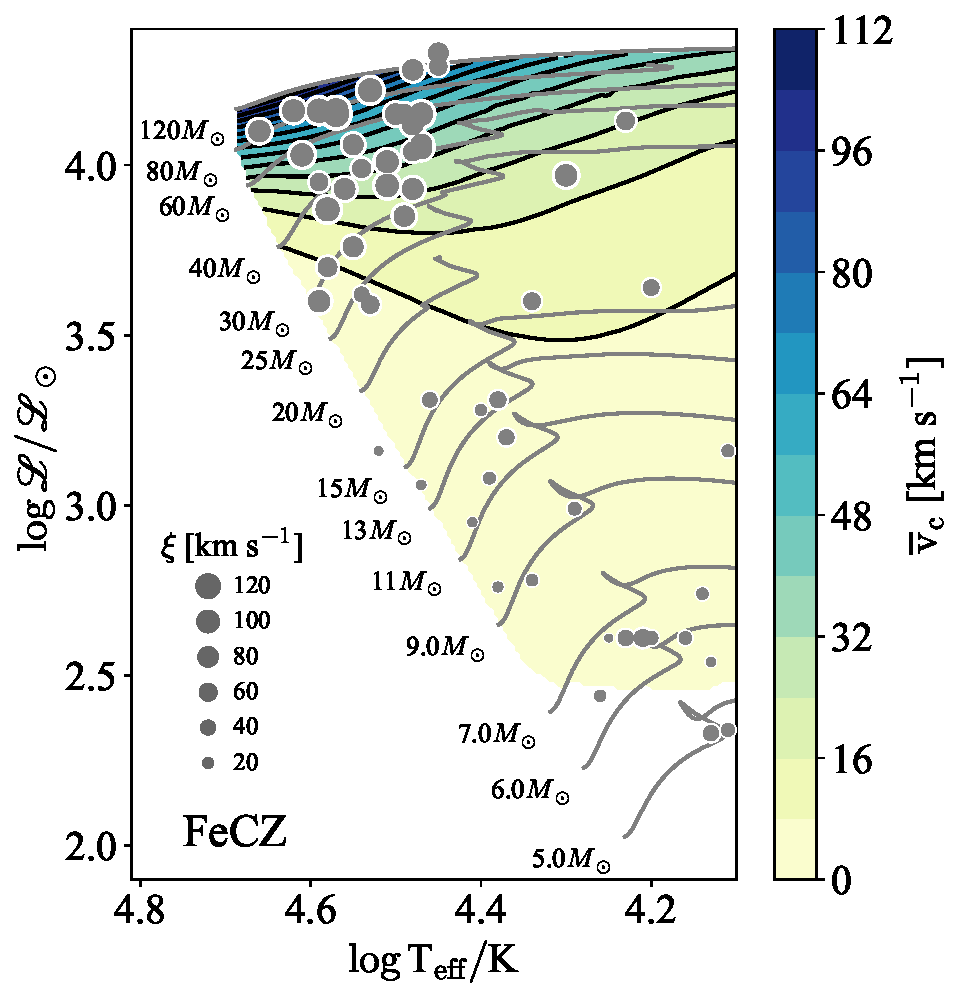
\includegraphics[width=1.0\columnwidth]{../figures/vc_FeCZ_macroturbulence.pdf}
\caption{\label{fig:nuchar_fecz} Average convective velocities in the FeCZ  as function of the location of stellar models in the spectroscopic H-R Diagram. We also show the observed stars with detected macroturbulent velocity as grey dots. The size of the dot is proportional to the observed macroturbulence.}
\end{center}
\end{figure}


\subsection{Subsurface Convection and Photometric Variability}

\begin{figure*}[htp]
  \centering
  \subfloat{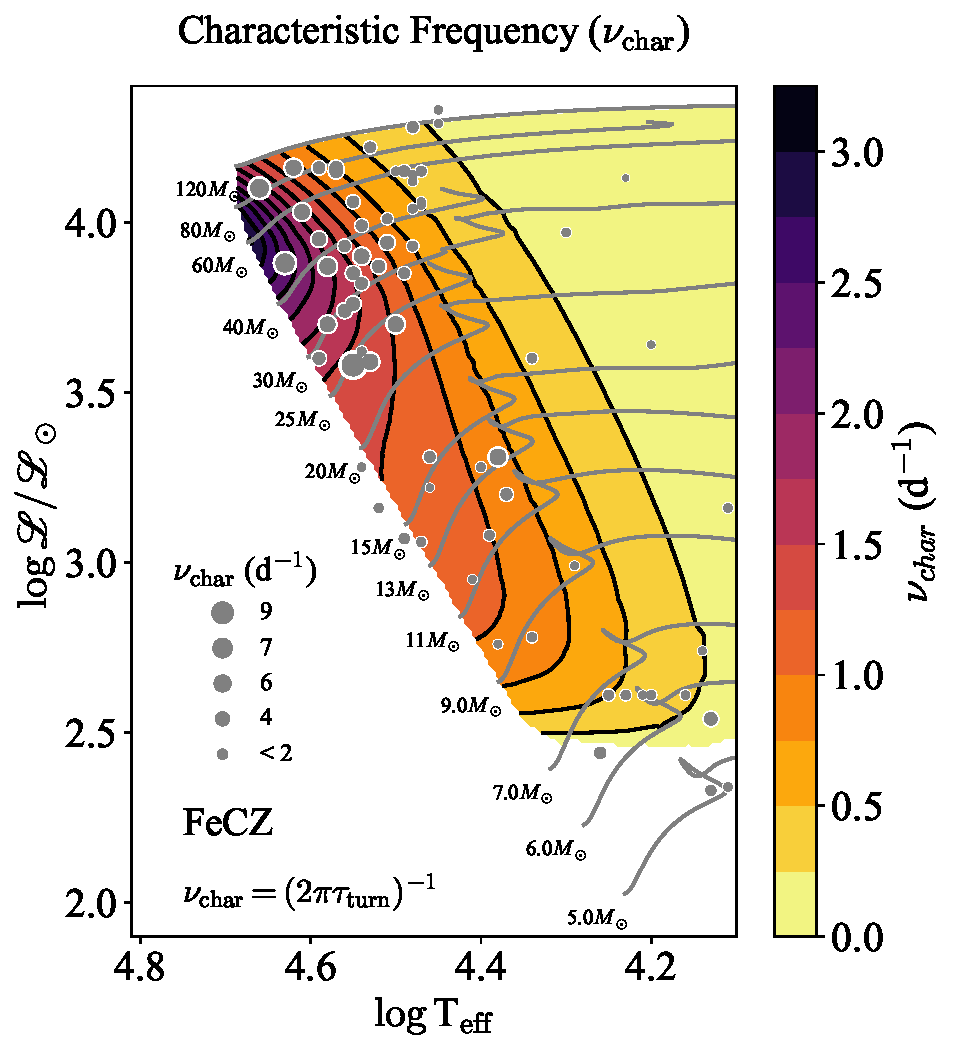
\includegraphics[width=1\columnwidth]{../figures/freq_FeCZ_data.pdf}}\hfill
  \subfloat{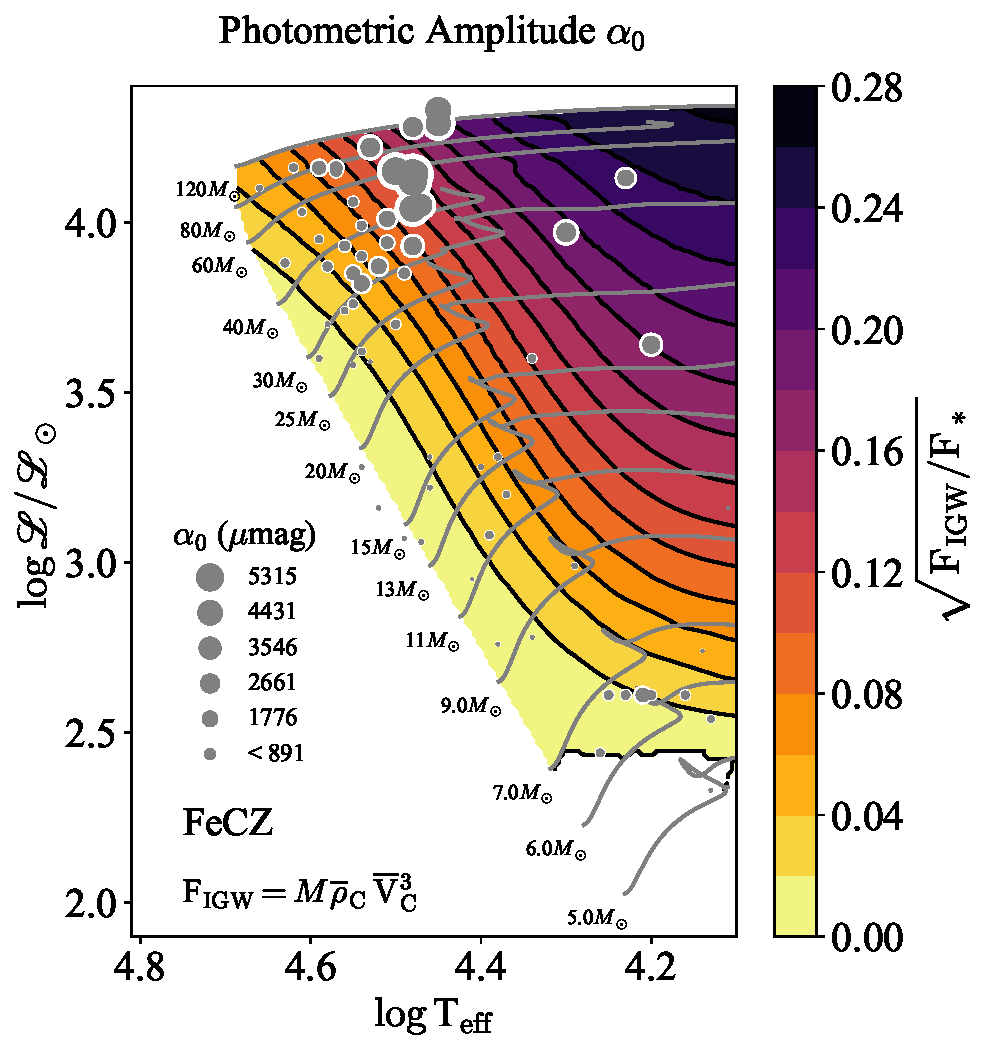
\includegraphics[width=1.04\columnwidth]{../figures/sqrt_flux_FeCZ_mach_rednoise.pdf}}
   \caption{ Left panel: Characteristic frequency $\nu_{\rm char}$ in the FeCZ as a function of the location of stellar models in the spectroscopic H-R Diagram. We also show the observed stars with detected stochastic photometric variability as grey dots. The size of the dot is proportional to $\nu_{\rm char}$. Right panel: Flux of gravity waves launched by the FeCZ divided by total stellar flux. The IGWs flux is calculated multiplying the convective flux in the FeCZ by the average convective Mach number (this is calculated in the top pressure scale height of the convective region). We also show the observed stars with detected stochastic photometric variability as grey dots. The size of the dot is proportional to $\alpha_0$.}
    \label{fig:nuchar_core}
\end{figure*}







\subsection{Core Convection and Photometric Variability}


\begin{figure*}[htp]
  \centering
  \subfloat{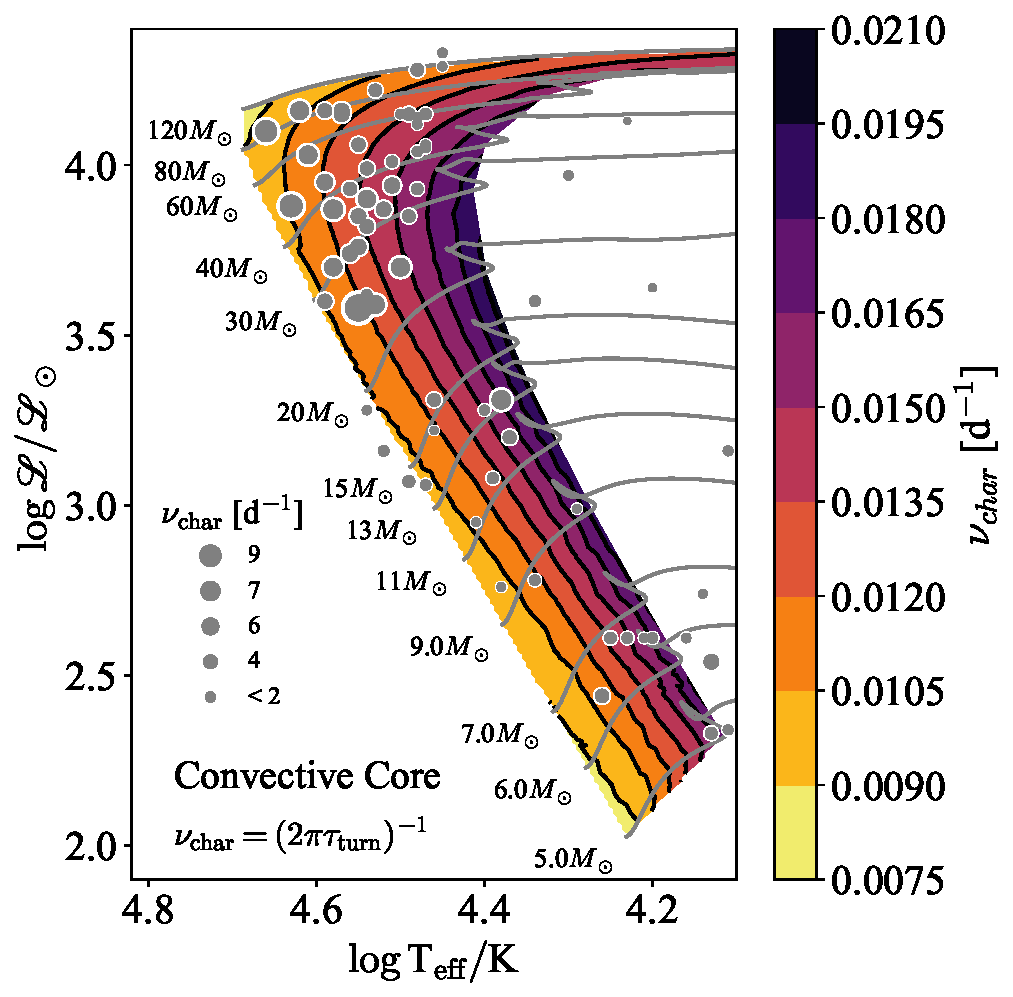
\includegraphics[width=1\columnwidth]{../figures/freq_core_data_days.pdf}}\hfill
  \subfloat{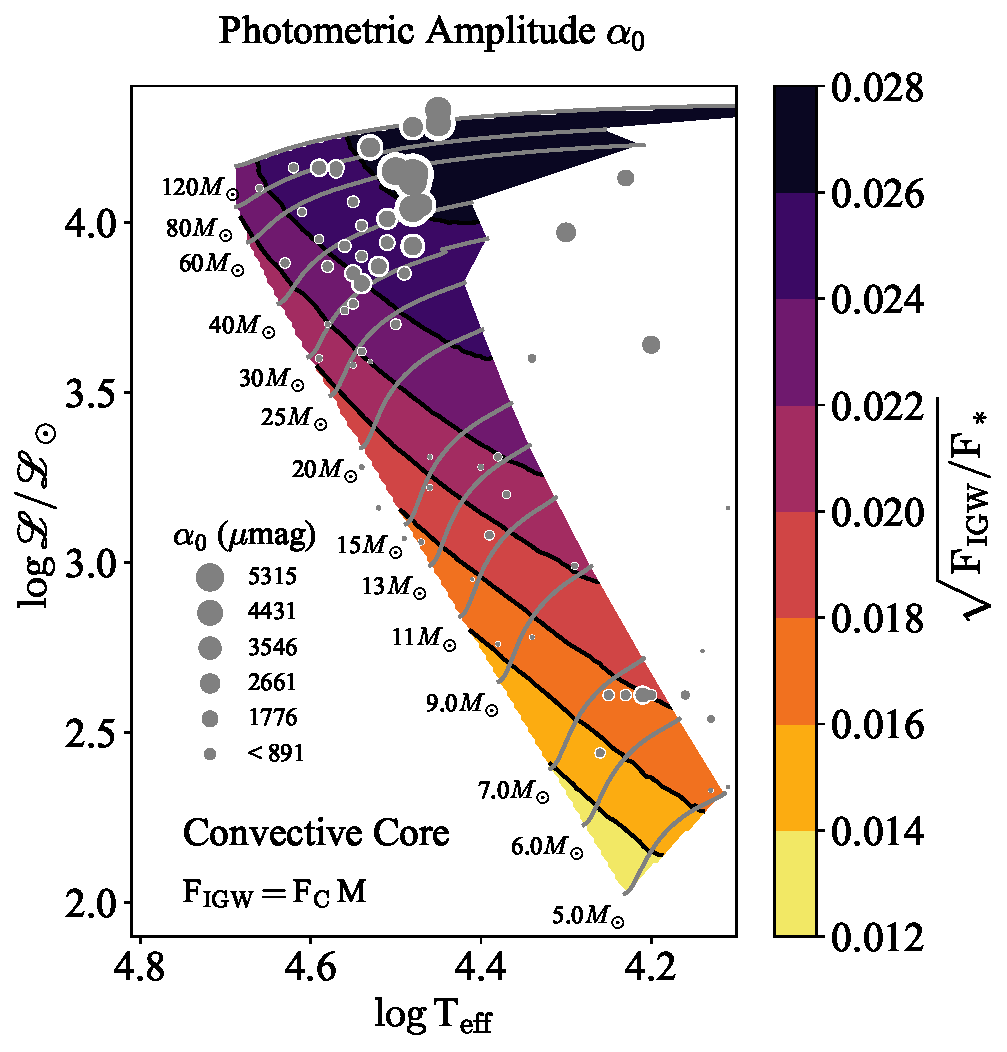
\includegraphics[width=1.02\columnwidth]{../figures/relative_flux_IGW_ahp_core_rednoise_data.pdf}}
   \caption{ Left panel: Characteristic frequency $\nu_{\rm char}$ in the convective core as function of the location of stellar models in the spectroscopic HRD. We also show the observed stars with detected stochastic photometric variability as grey dots. The size of the dot is proportional to $\nu_{\rm char}$. Right panel: Flux of gravity waves launched by the convective core. This is calculated multiplying the convective flux in the core by the average convective Mach number (this is calculated in the top pressure scale height of the convective region). We also show the observed stars with detected stochastic photometric variability as grey dots. The size of the dot is proportional to $\alpha_0$.}
    \label{fig:nuchar_core}
\end{figure*}


\subsection{A unified model for surface phenomena in massive stars}
The presence of subsurface convection can simultaneously account for a large variety of puzzling phenomena that appear ubiquitous at the surface of early-type stars.
First of all we have microturbulence and macroturbulence. Both can be accounted for by velocity fields excited by the underlying FeCZ subsurface convection zone (Cantiello2009, Grassitelli 2015, This work).
Photospheric magnetic spots: These spots might cause the ubiquitous DACs, resulting from CIRs in the winds of massive stars.
The seed of wind clumping. 
Finally, the presence of a turbulent velocity field necessarily has to induce photometric variability, and we have shown here that the observed low-frequency stochastic noise observed observed in the majority of massive stars correlates very well with the presence and properties of the FeCZ. 
As such, a minimal hypothesis is that the presence of the FeCZ is the underlying physical cause and represent a possible unified model for the appearance of turbulence, magnetic spots, low-frequency photometric variability and wind structure and variability in massive stars. 

\subsection{Conclusions}



\begin{figure}[ht!]
\begin{center}
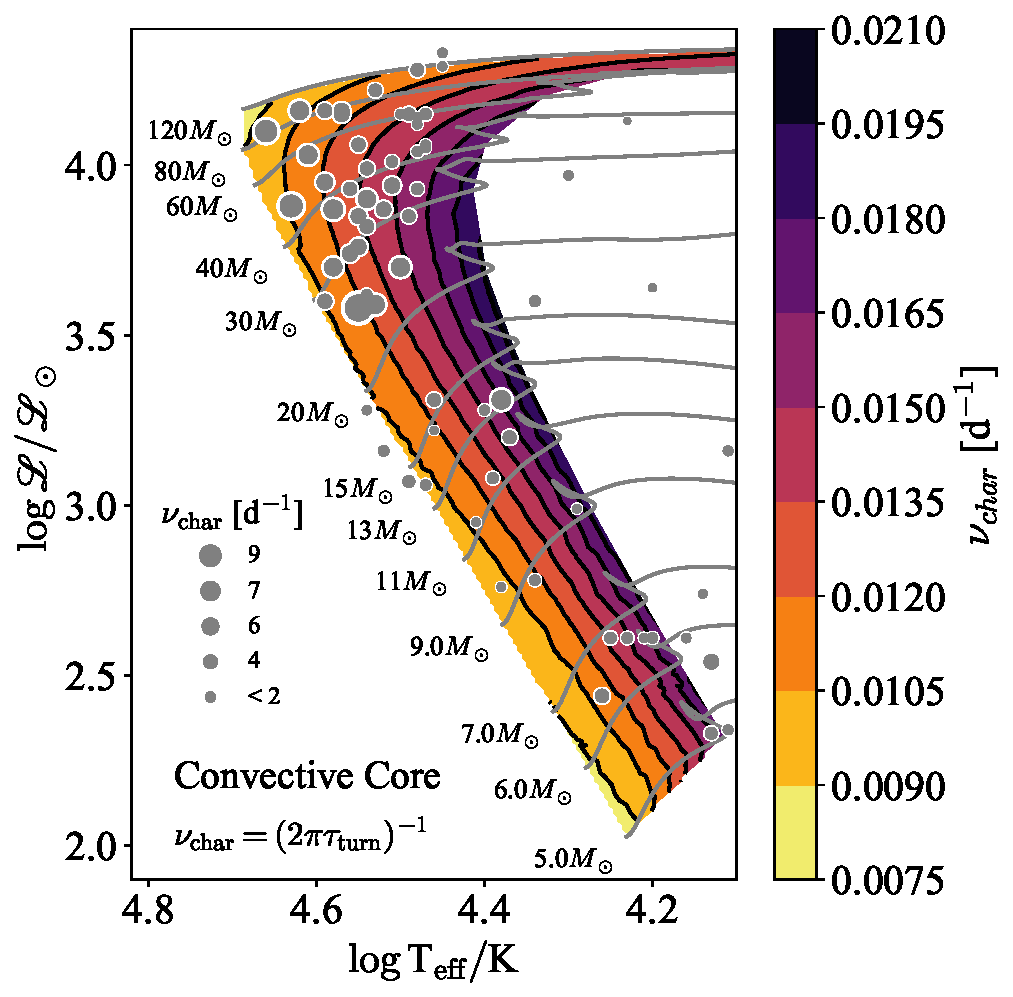
\includegraphics[width=1.0\columnwidth]{../figures/freq_core_data_days.pdf}
\caption{\label{fig:nuchar_core} Characteristic frequency $\nu_{\rm char}$ in the convective core as function of the location of stellar models in the spectroscopic HRD. We also show the observed stars with detected stochastic photometric variability as grey dots. The size of the dot is proportional to $\nu_{\rm char}$.}
\end{center}
\end{figure}


%\begin{figure}[ht!]
%\begin{center}
%\includegraphics[width=1.0\columnwidth]{../figures/flux_IGW_ahp_core_rednoise_data.pdf}
%\caption{\label{fig:alpha0_core_igw} Flux of gravity waves launched by the convective core. This is calculated multiplying the convective flux in the core by the average convective Mach number (this is calculated in the top pressure scale height of the convective region). We also show the observed stars with detected stochastic photometric variability as grey dots. The size of the dot is proportional to $\alpha_0$.}
%\end{center}
%\end{figure}



\begin{figure}[ht!]
\begin{center}
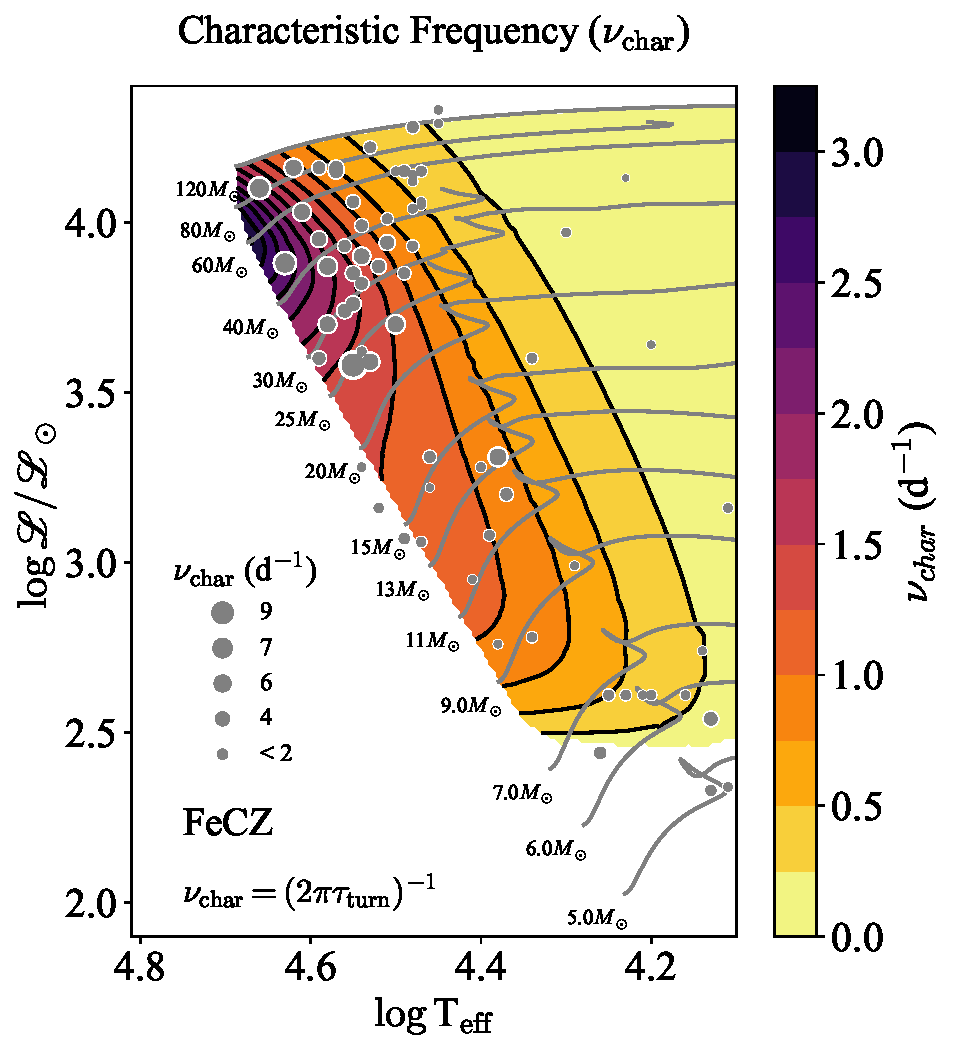
\includegraphics[width=1.0\columnwidth]{../figures/freq_FeCZ_data.pdf}
\caption{\label{fig:nuchar_fecz} Characteristic frequency $\nu_{\rm char}$ in the FeCZ as a function of the location of stellar models in the spectroscopic H-R Diagram. We also show the observed stars with detected stochastic photometric variability as grey dots. The size of the dot is proportional to $\nu_{\rm char}$.}
\end{center}
\end{figure}


%\begin{figure}[ht!]
%\begin{center}
%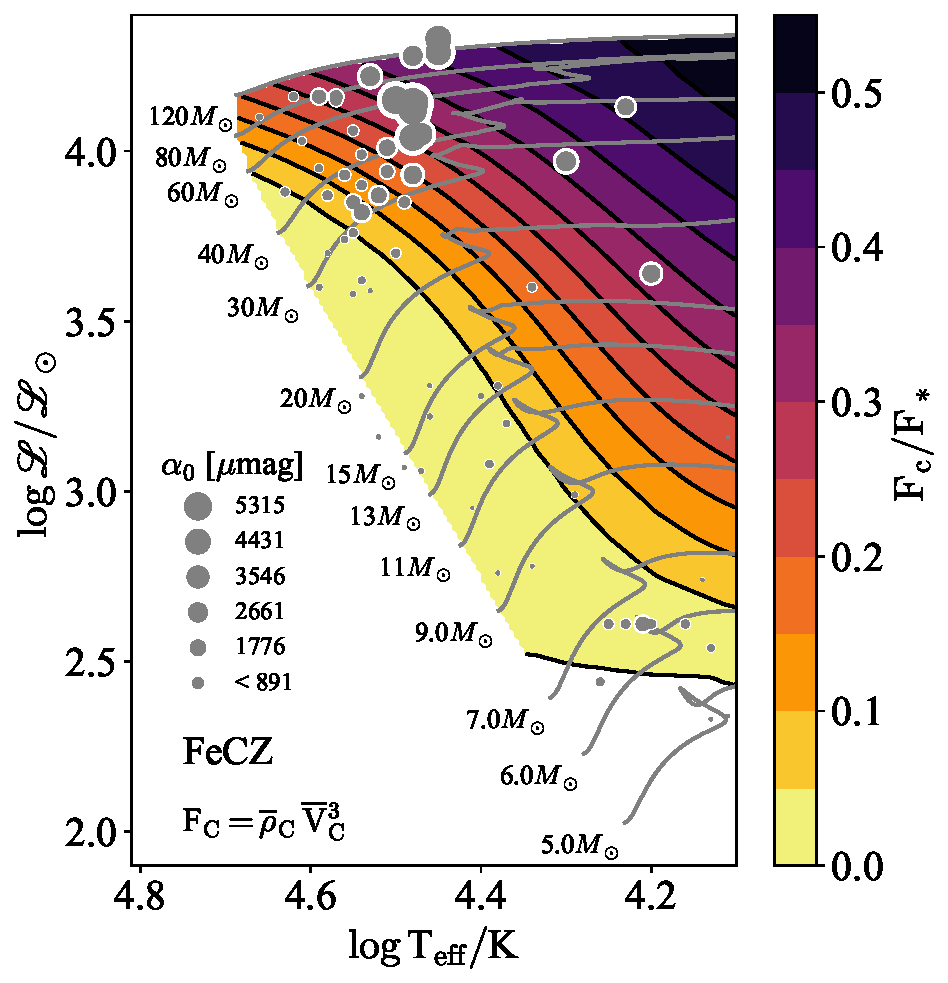
\includegraphics[width=1.0\columnwidth]{../figures/flux_FeCZ_rednoise.pdf}
%\caption{\label{fig:alpha0_flux} Maximum convective flux in the FeCZ divided by the total stellar flux in the spectroscopic H-R Diagram. We also show the observed stars with detected stochastic photometric variability as grey dots. The size of the dot is proportional to $\alpha_0$.}
%\end{center}
%\end{figure}


\begin{figure}[ht!]
\begin{center}
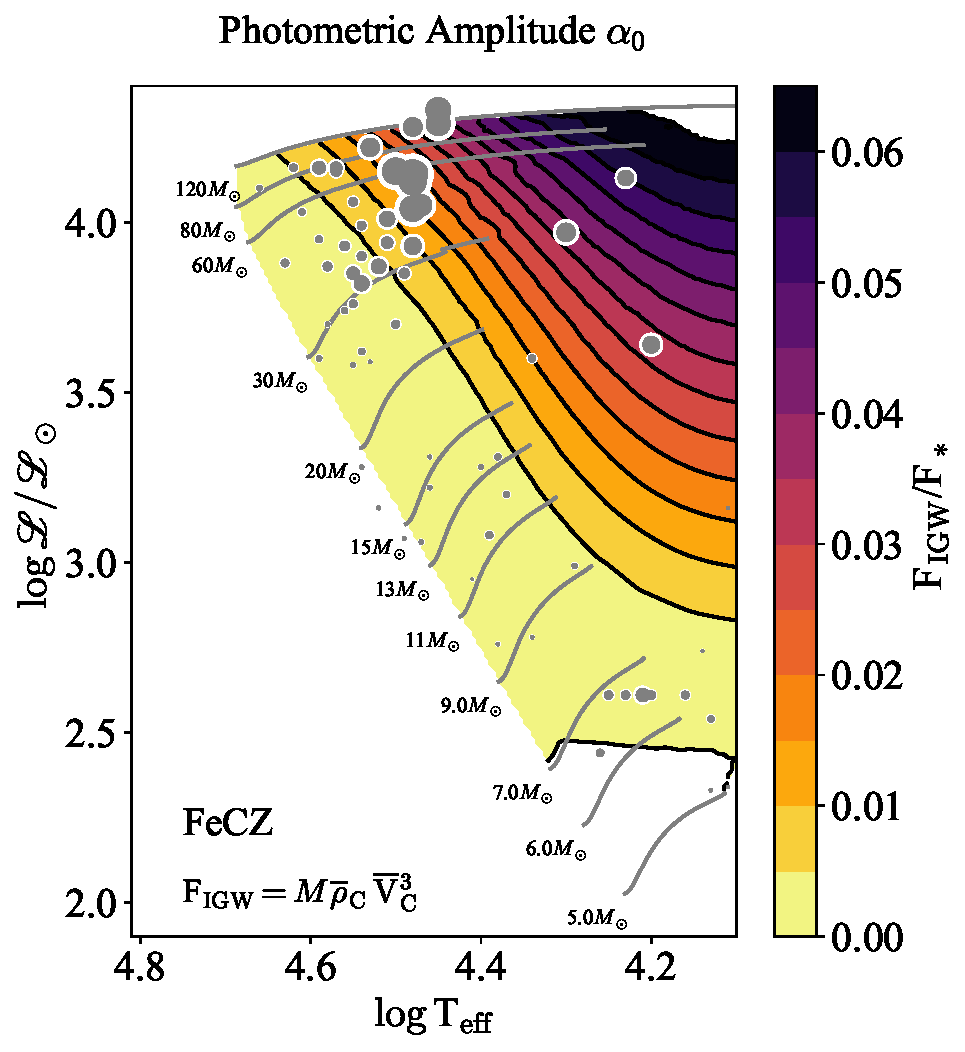
\includegraphics[width=1.0\columnwidth]{../figures/flux_FeCZ_mach_rednoise.pdf}
\caption{\label{fig:alpha0_flux_igw} Flux of gravity waves launched by the FeCZ. This is calculated multiplying the convective flux in the FeCZ by the average convective Mach number (this is calculated in the top pressure scale height of the convective region). We also show the observed stars with detected stochastic photometric variability as grey dots. The size of the dot is proportional to $\alpha_0$.}
\end{center}
\end{figure}



\begin{figure}[ht!]
\begin{center}
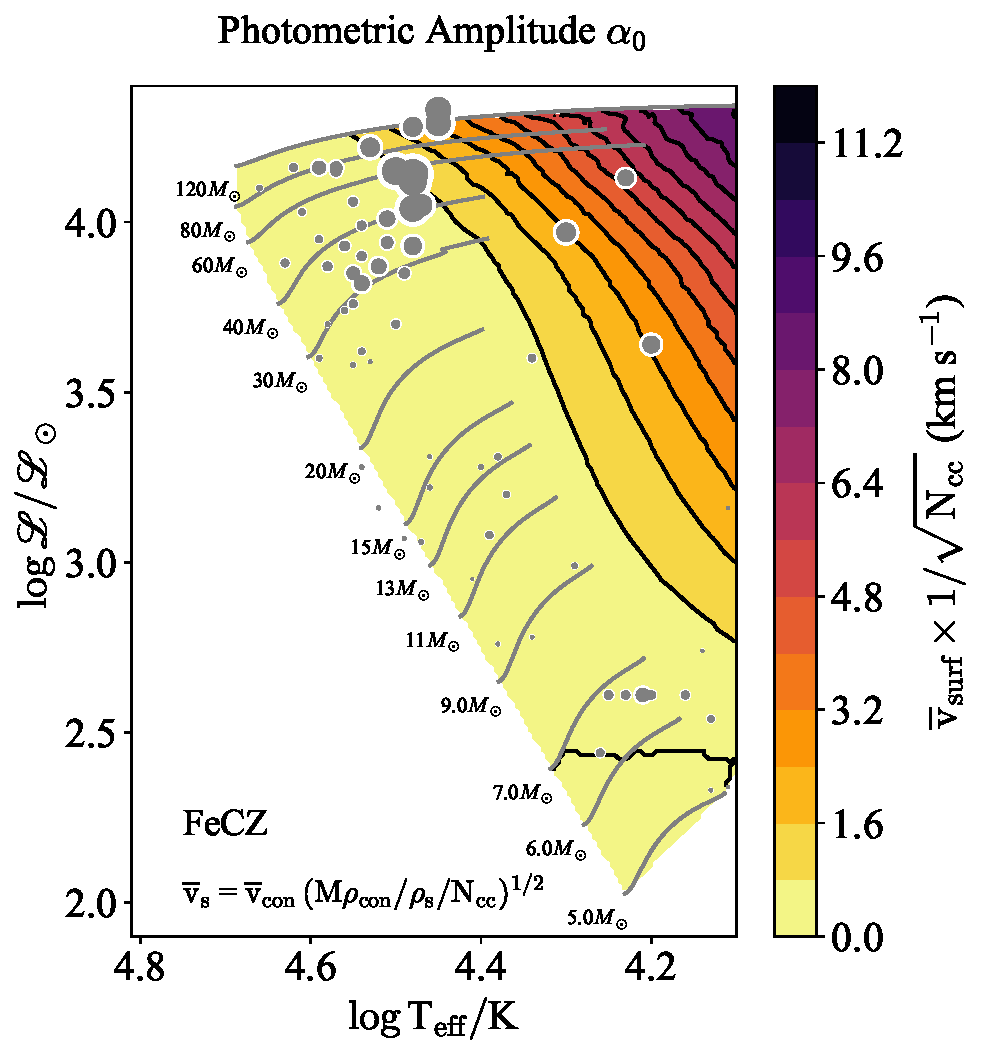
\includegraphics[width=1.0\columnwidth]{../figures/vsurf_ncells_FeCZ_data.pdf}
\caption{\label{fig:alpha0_vel_ncells} Reduced amplitude of velocity fluctuations at the stellar surface induced by internal gravity waves launched by the FeCZ in the spectroscopic H-R Diagram. After calculating the velocity fluctuation, we have corrected for cancellation effects dividing by the total number of convective cells. We also show the observed stars with detected stochastic photometric variability as grey dots. The size of the dot is proportional to $\alpha_0$.}
\end{center}
\end{figure}



\acknowledgments
The Center for Computational Astrophysics at the Flatiron Institute is supported by the Simons Foundation.
This research was supported in part by the National Science Foundation under Grant No. NSF PHY-1748958 and by the Gordon and Betty Moore Foundation through Grant GBMF7392

\appendix
\section{Software Details}
\label{sec:software}

Calculations were done with \code{MESA} version 11701.
The \code{MESA} EOS is a blend of the OPAL \citet{Rogers2002}, SCVH
\citet{Saumon1995}, PTEH \citet{Pols1995}, HELM
\citet{Timmes2000}, and PC \citet{Potekhin2010} EOSes.

Radiative opacities are primarily from OPAL \citep{Iglesias1993,
Iglesias1996}, with low-temperature data from \citet{Ferguson2005}
and the high-temperature, Compton-scattering dominated regime by
\citet{Buchler1976}.  Electron conduction opacities are from
\citet{Cassisi2007}.

Nuclear reaction rates are a combination of rates from
NACRE \citep{Angulo1999}, JINA REACLIB \citep{Cyburt2010}, plus
additional tabulated weak reaction rates \citet{Fuller1985, Oda1994,
Langanke2000}. Screening is included via the prescription of \citet{Chugunov2007}.
Thermal neutrino loss rates are from \citet{Itoh1996}.

The inlists, processing scripts, and model output are available at~\url{Zenodo.org}.


\bibliographystyle{aasjournal}
\bibliography{biblio.bib}

\end{document}
